\documentclass{ieeeojies}
\usepackage{cite}
\usepackage{amsmath,amssymb,amsfonts}
\usepackage{algorithmic}
\usepackage{graphicx}
\usepackage{textcomp}
\usepackage{array}
\usepackage[table]{xcolor}
\usepackage{multirow}
\usepackage{multicol}
\usepackage{float}
\usepackage{newunicodechar}

\newunicodechar{ℝ}{\mathbb{R}}

\def\BibTeX{{\rm B\kern-.05em{\sc i\kern-.025em b}\kern-.08em
    T\kern-.1667em\lower.7ex\hbox{E}\kern-.125emX}}
    

\begin{document}
\title{COMPARING ML/DL ALGORITHMS IN REAL ESTATE STOCK PRICES ANALYSIS AND PREDICTION}

\author{\uppercase{NGO THUY YEN NHI}\authorrefmark{1},
\uppercase{NGUYEN DUONG\authorrefmark{2}, PHAM DUY KHANH}\authorrefmark{3},
\uppercase{NGUYEN NGOC HA MY\authorrefmark{4}, \\ LE THUAN HIEU}\authorrefmark{5}}

\address[1]{Faculty of Information Systems, University of Information Technology, (e-mail: 21521230@gm.uit.edu.vn)}
\address[2]{Faculty of Information Systems, University of Information Technology, (e-mail: 21521990@gm.uit.edu.vn)}
\address[3]{Faculty of Information Systems, University of Information Technology, (e-mail: 21522211@gm.uit.edu.vn)}
\address[4]{Faculty of Information Systems, University of Information Technology, (e-mail: 21522351@gm.uit.edu.vn)}
\address[5]{Faculty of Information Systems, University of Information Technology, (e-mail: 21522072@gm.uit.edu.vn)}

\markboth
{Author \headeretal: Ngo Thuy Yen Nhi, Nguyen Duong, Pham Duy Khanh, Nguyen Ngoc Ha My, Le Thuan Hieu}
{Author \headeretal: Ngo Thuy Yen Nhi, Nguyen Duong, Pham Duy Khanh, Nguyen Ngoc Ha My, Le Thuan Hieu}

\begin{abstract}
\\
\textit{Machine learning and deep learning techniques is renowned for playing a pivotal role in the realm of Business Analytics nowadays by leveraging time-series datasets with the aspiration to provide businesses with analytics-driven insights that assist in facilitating decision-making, improve performance, and optimize processes. Due to the rapid and diverse development of algorithms, there aries a critical need to scrutinize the efficacy of them within specific domains. This paper addresses this imperative by utilizing and evaluating five distinct algorithms - FEDformer, TBATS, AR-MOS, Kalman Filter, and ResNet towards three different time-series datasets from three distinguished real estate companies in Viet Nam. Within the context of this study, the objective is to analyze and forecast the trajectory their stock prices based on their historical daily stock price records. The study delves into an extensive comparative analysis of these algorithms' capabilities and outlines a detailed methodology that illuminates the intricacies of each algorithm's application and the rationale behind their selection. Subsequently, the study applies the findings obtained from the completed analyses to elucidate the strengths and limitations of each approach. Ultimately, through systematic rigorous evaluation and comparison, this paper aims to enhance the understanding of the suitability and competently of these algorithms for stock prices analysis and prediction within the real estate domain in Viet Nam.}
\end{abstract}

\begin{keywords}
\\
\textit{Analytic, AR-MOS, Comparison, Efficacy, 
FEDformer, Kalman Filter, Market capitalization,
Prediction, Real estate, ResNet, Stock prices, TBATS, Time-series.}
\end{keywords}

\titlepgskip=-15pt

\maketitle

\section{Introduction}
\label{sec:introduction}
In the contemporary era shaped by rapid societal and technological advancements, a typical modern business or industrial organization is constantly in demand of a cutting-edge and robust analytical tools for effective decision-making and risk management. Therefore, there arises a pressing need for advanced analytical tools and methodologies to navigate and extract insights from vast volumes of data.\\ 
In general, the world, and specifically Viet Nam, the real estate sector has experienced rapid growth and transformation in recent years, driven by urbanization, economic development, and foreign investment. Amidst this dynamic landscape, accurate estate analysis and forecasting play a pivotal role in facilitating informed decision-making and strategic planning for real estate companies. Stock prices, as a key indicator of a company's value and performance, serves as a crucial metric for investors, analysts, and industry stakeholders alike. Accurate prediction of market capitalization not only aids investors in decisions making but also assists real estate companies in strategizing their operations and investments effectively. \\
Given the importance need for robust analysis and predictive models within the real estate domain in Viet Nam, Machine learning and Deep learning techniques have emerged as powerful tools in this regard, offering the potential to uncover patterns, trends, and predictive signals within time-series datasets. Against this backdrop, this study investigates the capabilities of various machine learning and deep learning algorithms in analyzing and forecasting stock prices for three prominent real estate companies in Vietnam (DXG, DIG and NVL). Ultimately, the objective is to elucidate the efficacy and comparative performance between the five methodologies of ML/DL algorithms - FEDformer, TBATS, AR-MOS, Kalman Filter, and ResNet by leveraging three different time-series datasets based on historical daily stock price records of those three Vietnamese prominent real estate companies. \\
The primary goal of this paper is twofold as it embarks on a comprehensive examination of the five algorithms methodologies: \\
Firstly, to evaluate the performance and effectiveness of the five selected algorithms in analyzing and forecasting daily stock price data for the specified real estate companies.
Secondly, to conduct a comparative analysis of their efficacy and performance, highlighting the strengths as well as limitations of each approach, and examine the suitability and competency of these algorithms in the context of real estate market analysis. \\
The structure of this paper is organized to provide a comprehensive understanding of these objectives to outline the suitability and competency of these algorithms. Following this introduction, the subsequent section – Related Work, reviews existing literature and research relevant to ML/DL applications in real estate analysis. Then, the Material section provides the dataset descriptions, data selection criteria, and descriptive statistics employed in this study. Subsequently, in the Methodology section, the study presents the criteria for algorithm selection, and the evaluation metrics utilized in this investigation. In the following section, the Results section presents the findings derived from the application of each algorithm and the evaluation methods deployed. Finally, the Conclusion section summarizes the key findings, discusses their implications, and outlines avenues for future considerations.


\section{Related Works}

% In recent years, there has been a substantial amount of research dedicated to predicting stock prices using various machine learning and statistical models. \\
% V. Gururaj, in a 2019 study \cite{b1}, focused on stock market prediction employing Linear Regression and Support Vector Machines, demonstrating the application of these models in forecasting stock prices.\\
Stock prices can be influenced due to various factors such as company’s status, market sentiment, or economic indicators, etc. In recent years, a plethora of studies had been dedicated for analysing and predicting stock prices, employing a variety of ML/DL algorithms, and statistical models. The methodologies encompass statiscal and analytical approaches achieved through a diverse selection of those ML/DL techniques and hybrid forecasting methods.\\ 
Therefore, this section focuses on critically examining existing literatures and research papers pertinent to the comparative performance of various ML/DL algorithms as well as statistical models’ applications in stock price analysis and prediction. The aim is to contextualize recent studies, identifying key trends, methodologies, and findings in the field and provide an overview of the ML/DL algorithms used in this work comparing with others in different scenarios. This will assist further investigation and provide suggested selection of methodologies applied in the study to evaluate and determine the efficacy of each ML/DL algorithms and models utilized in this research.\\
A research article released in 2023 by Agus Tri Haryono, Riyanarto Sarno, and Kelly Rossa Sungkono suggested that the architecture of FEDformer, another transformer of time-series, outperformed its counterparts such as AutoFormer, Informer, and Reformer in predicting stock prices. Additionally, the performances of AutoFormer, Informer, and Reformer were also stated to be more advanced compared to ARIMA and LSTM models. For stock prices forecasting, the evaluation methods deployed including R2, RMSE, MSE, and MAPE with the time lag variants of 5, 10, 20, 100, and 200 for a specified stock issuer. The outcomes revealed that FEDformer possessed a superior efficacy with an RMSE score 83.08\% lower than Transformer and 84.83\% lower than Informer. Futhermore, the MAPE score of FEDformer was also 85.17\% lower than Transformer and lower by 96.66\% compared to Informer. Without a doubt, FEDformer emerges as a dominant selection among other transformer models in resolving limitations on trend capture in long-term time series forecasting.
Another study conducted in 2022 by Sasha S. Yamada and Ogulcan E. Örsel issued an efficacy comparison between a linear Kalman filter and different varieties of LSTM to forecast future stock prices based on historical stock prices data spanning on a 10-year period. The research found that the accuracy of each model is significantly influenced by the volatility of the stock being forecasted. With the training dataset consisting of 7.5 years of historical stock prices, the testing set used used to predict next-day stock prices consists of 2.5 years of prices. By applying RMSE and MAE evaluation method, the findings showed that Kalman Filter demonstrated an RMSE score of 62.67\% and MAE score of 87.65\% higher than average RMSE and MAE score of different LSTM variances. As a result, for low-volatility stocks, a linear Kalman filter can predict next-day prices with very reasonable accuracy. However, this error increases significantly for greater volatile stocks, making LSTM architectures a much more suitable choice for forecasting in such scenarios.\\
In a blog published in 2021 by Nadeem, the efficacy of TBATS models in stock prices time-series forecasting was proposed, compared with SARIMA and SARIMAX with 2 Fourier Terms. By utilizing MAE evaluation method, the study indicated the dominance of TBATS with an MAE score of 46.6\% and 1.19\% lower than the other 2 models. Although TBATS still possesses a few drawbacks as it can slow the computation down, this model is preferable when dealing with time-varying seasonality and is user-friendly for handling data with multiple seasonal patterns.\\
In a study conducted by Bowen Song and Heng Liu in 2018 titled “Stock Price Trend Prediction Model Based on Deep Residual Network and Stock Price Graph”, ResNet model was introduced for stock prices prediction and exhibited the average accuracy of 0.40, which surpassed the stochastic indicator of 0.33 when using the stock price graph as input. The paper compared the ResNet model with three selected widely used financial time-series prediction models: SVM, DNN, and CNN. Overall, ResNet and CNN variants demonstrated the highest accuracy and showcased the most stablility in the classifier evaluation index. The deep learning models, such as ResNet, CNN, and DNN, were found to be superior to SVM due to their ability to capture the hidden dynamics of stocks with their complex network structure. Additionally, CNN and ResNet filter features through convolution operations, optimize the learning process, and mitigate overfitting compared to DNN, thereby improving accuracy.\\
Collectively, these studies contribute to the increasing collection of literature on ML/DL applications in real estate stock price prediction, exhibiting the versatility and effectiveness of various models across different market conditions and time frames. By synthesizing key findings and methodologies, this section provides a comprehensive overview of the state-of-the-art techniques and avenues for future research in the field.


\section{Materials}
\subsection{Dataset}

In this article, we scrutinize the stock prices data of three following prominent real estate companies in Viet Nam:
\begin{itemize}
    \item Dat Xanh Group (DXG), 
    \item Development Investment Construction JSC (DIG),
    \item No Va Land Investment Group Corporation (NVL).
\end{itemize} \\
Each dataset presents a record of each company's stock prices, thoroughly documented spanning from January 1, 2018, to March 22, 2024, with a daily time frame on trading activities. These datasets are sourced from Investing.com, a reputable financial platform renowned for providing comprehensive trading information for companies or financial organization.\\
The datasets feature the following array of variables, providing crucial insights and materials for the study. The variables include:
\begin{itemize}
    \item Date: Presenting the trading date in the format DD/MM/YYYY.
    \item Price: Denoting the closing price of the stock on the respective trading day.
    \item Open: Signifying the opening price of the stock on the respective trading day.
    \item High: Presenting the highest recorded of the stock price within the trading day.
    \item Low: Indicating the lowest recorded of the stock price during the trading period.
    \item Vol: Evaluating the trading volume for each day, represented by the number of shares traded (expressed in millions of shares).
    \item Change (\%): Determining the percentage change in the stock's value compared to the preceding trading day.
\end{itemize} \\
All data referring to stock-related metrics are denominated in Vietnamese Dong (VND), ensuring consistency and coherence throughout the analysis.

\subsection{Descriptive Statistics}
\begin{table}[H]
  \centering
  \caption{DXG, DIG, NVL’s Descriptive Statistics}
\begin{tabular}{|>{\columncolor{red!20}}c|c|c|c|}
    \hline
     \rowcolor{red!20} & DIG & DXG & NVL \\ \hline
     Count & 1552 & 1552 & 1552 \\ \hline
     Mean & 20575.539 & 17846.990 & 41771.515\\ \hline
     Std & 16677.794 & 7144.933 & 23474.855\\ \hline
     Min & 6591.800 & 6739.100 & 10250\\ \hline
     25\% & 8852.700 & 12814.250 & 28928\\ \hline
     50\% & 14799.700 & 17000 & 34248\\ \hline
     75\% & 25800 & 20586.350 & 60244.250\\ \hline
     Max & 98196.700 & 46750 & 92366\\ \hline
\end{tabular}
\end{table}

\begin{figure}[H]
    \centering
    \begin{minipage}{0.23\textwidth}
    \centering
    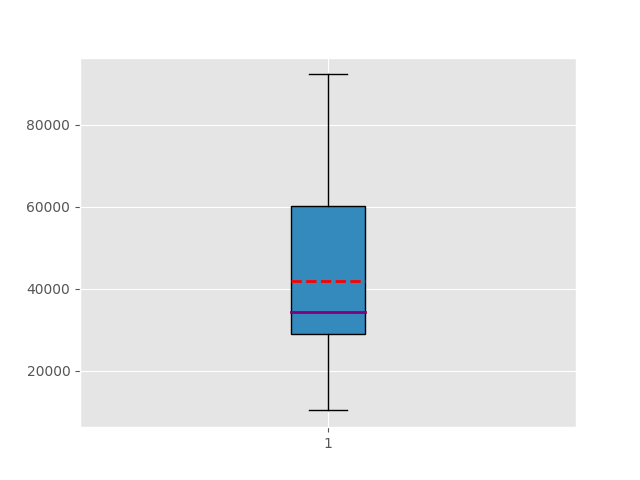
\includegraphics[width=1\textwidth]{Boxplot_NVL.png}
    \caption{NVL stock price's boxplot}
    \label{fig:1}
    \end{minipage}
    \hfill
    \begin{minipage}{0.23\textwidth}
    \centering
    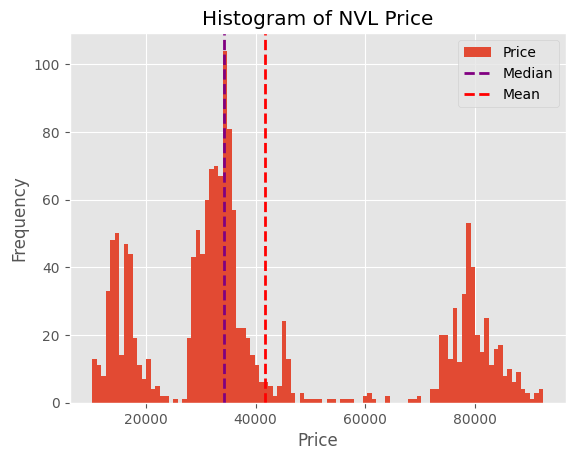
\includegraphics[width=1\textwidth]{Histogram NVL.png}
    \caption{NVL stock price's histogram}
    \label{fig:2}
    \end{minipage}
\end{figure}

\begin{figure}[H]
    \centering
    \begin{minipage}{0.23\textwidth}
    \centering
    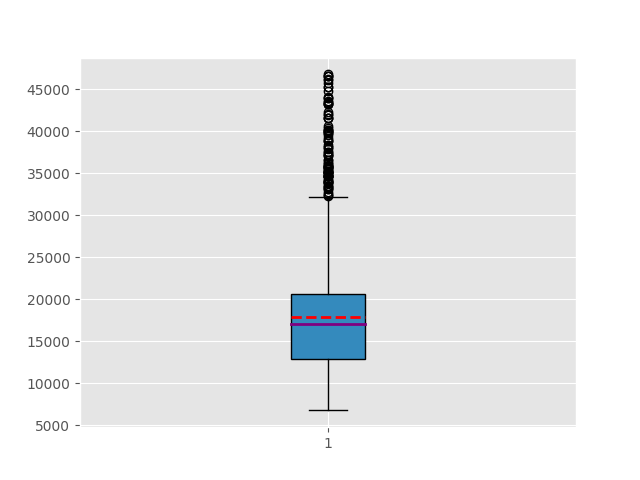
\includegraphics[width=1\textwidth]{Boxplot_DXG.png}
    \caption{DXG stock price's boxplot}
    \label{fig:1}
    \end{minipage}
    \hfill
    \begin{minipage}{0.23\textwidth}
    \centering
    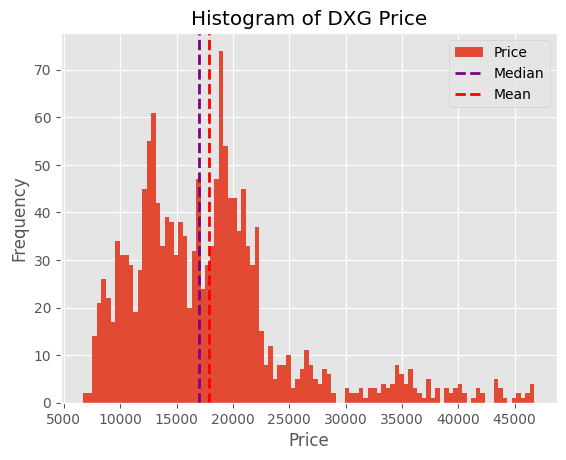
\includegraphics[width=1\textwidth]{Histogram DXG.png}
    \caption{DXG stock price's histogram}
    \label{fig:2}
    \end{minipage}
\end{figure}

\begin{figure}[H]
    \centering
    \begin{minipage}{0.23\textwidth}
    \centering
    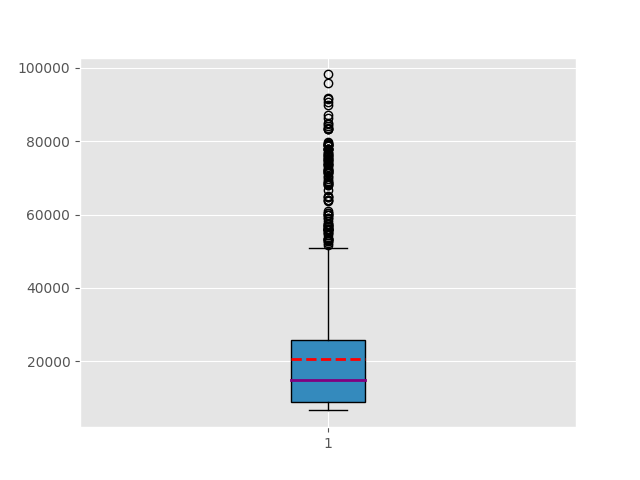
\includegraphics[width=1\textwidth]{Boxplot_DIG.png}
    \caption{DIG stock price's boxplot}
    \label{fig:1}
    \end{minipage}
    \hfill
    \begin{minipage}{0.23\textwidth}
    \centering
    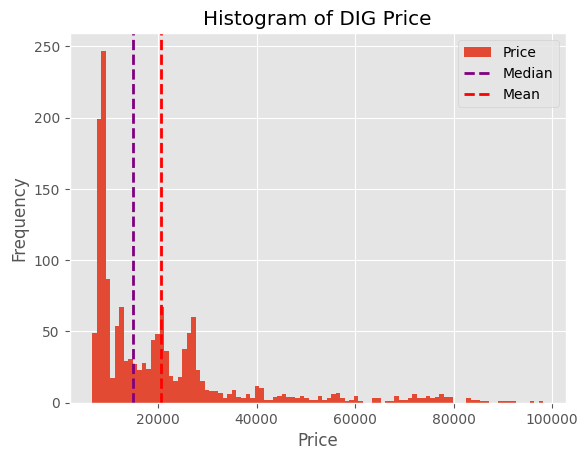
\includegraphics[width=1\textwidth]{Histogram DIG.png}
    \caption{DIG stock price's histogram}
    \label{fig:2}
    \end{minipage}
\end{figure}

\section{Methodology}
%\subsection{Linear Regression}
%Regression analysis is a tool for building mathematical and statistical models that characterize relationships between a dependent variable and one or more independent, or explanatory, variables, all of which are numerical. This statistical technique is used to find an equation that best predicts the y variable as a linear function of the x variables.
% A multiple linear regression model has the form: 
% \[Y=\beta_0+\beta_1X_1+\beta_2X_2+\cdots+\beta_kX_k+\varepsilon\]
% Where:\\
% 	\indent\textbullet\ Y is the dependent variable (Target Variable).\\
% 	\indent\textbullet\ \(X_1, X_2, \ldots, X_k\) are the independent (explanatory) variables.\\
% 	\indent\textbullet\ \(\beta_0\) is the intercept term.\\
% 	\indent\textbullet\ \(\beta_1,..., \beta_k\) are the regression coefficients for the independent variables.\\
% 	\indent\textbullet\ \(\varepsilon\) is the error term.
 

\section{Result}
\subsection{Evaluation Methods}
% \textbf{Mean Percentage Absolute Error} (MAPE): is the average percentage error in a set of predicted values.\\
% \[MAPE=\frac{100\%}{n}  \sum_{i=1}^{n} |y_i-\hat{y_i} |  = 1 \]\\
% \textbf{Root Mean Squared Error} (RMSE): is the square root of average value of squared error in a set of predicted values.\\
% \[RMSE=\sqrt{\sum_{i=1}^{n} \frac{(\hat{y_i}-y_i )^2}{n} }\]\\
% \textbf{Mean Absolute Error} (MSLE):is the relative difference between the log-transformed actual and predicted values.\\
% \[MSLE=\frac{1}{n}\sum_{i=1}^{n}(log(1+\hat{y_i})-log(log(1+y_i))^2\]
% Where: \\
% 	\indent\textbullet\ \(n\) is the number of observations in the dataset.\\
% 	\indent\textbullet\ \(y_i\)  is the true value.\\
% 	\indent\textbullet\ \(\hat{y_i}\) is the predicted value.
\subsection{DXG Dataset} 
% \begin{table}[H]
%     \centering
%     \begin{tabular}{|c|c|c|c|c|}
%          \hline
%          \multicolumn{5}{|c|}{\textbf{VCB Dataset's Evaluation}}\\
%          \hline
%          \centering Model & Training:Testing & RMSE & MAPE (\%) & MSLE\\
%          \hline
%          \multirow{2}{*}{LN} & 7:3 & 10508.77 & 10.71 & 0.015 \\ & 8:2 & 11729.2 & 10.825 & 0.019 \\ & \textbf{9:1} & \textbf{7933.49} & \textbf{7.47} & \textbf{0.007}\\
%          \hline
%          \multirow{2}{*}{SVR} & 7:3&11864.3&7.52&0.021\\ & 8:2&8521.33&5.01&0.009 \\ & \textbf{9:1} & \textbf{7006.54} & \textbf{3.73} & \textbf{0.006}\\
%          \hline
%          \multirow{2}{*}{GRU} & \textbf{7:3}	& \textbf{1545.676} & \textbf{1.262} & \textbf{0.00033} \\ & 8:2 & 1616.817 & 1.267 & 0.00035 \\ & 9:1 & 1699.655  & 1.052 & 0.00032\\
%          \hline
%          \multirow{2}{*}{ARIMA} & 7:3 &  8620.284 &  8.559 & 0.01 \\ & 8:2 &  11729.2 & 10.825 & 0.019 \\ & \textbf{9:1} & \textbf{7644.773}  & \textbf{7.287} & \textbf{0.007}\\
%          \hline
%          \multirow{2}{*}{SARIMA} & \textbf{7:3}	& \textbf{7971.644} & \textbf{7.755} & \textbf{0.009} \\ & 8:2 & 11711.484 & 10.809 & 0.019 \\ & 9:1 & 8629.708 & 8.253 & 0.009\\
%          \hline
%          \multirow{2}{*}{DLM} & 7:3 & 13156.831&13.336 & 0.021 \\ & \textbf{8:2} &	\textbf{7209.84} & \textbf{7.093} & \textbf{0.007} \\ & 9:1 &11945.338	&11.444&0.016\\
%          \hline
%          \multirow{2}{*}{SES} & 7:3 & 10949.0750 & 9.4738 & 0.0169 \\ & 8:2 & 11717.8586 &10.8142 & 0.0189 \\ & \textbf{9:1} &  	\textbf{6000.7953} &	\textbf{5.2412} & 	\textbf{0.004} \\
%          \hline
%          \multirow{2}{*}{BaggingGRU} & 7:3 & 941.7588 &  1.7384 &  0.0005 \\ & 8:2 & 939.7588 &  1.6546 &  0.0005 \\ & \textbf{9:1} & \textbf{936.8374} & \textbf{1.6273} & \textbf{0.0005}\\
%          \hline
%     \end{tabular}
%     \caption{VCB Dataset's Evaluation}
%     \label{vcbresult}
% \end{table}

% \begin{figure}[H]
%   \centering
%   \begin{minipage}{0.8\linewidth}
%     \centering
%     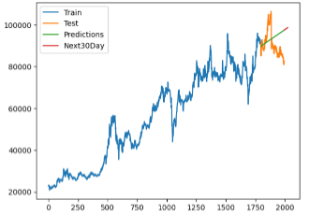
\includegraphics[width=\linewidth]{bibliography/LN_VCB91.png}
%     \caption{Linear model's result with 9:1 splitting proportion}
%     \label{fig8}
%   \end{minipage}
% \end{figure}
% \begin{figure}[H]
%   \centering
%   \begin{minipage}{0.8\linewidth}
%     \centering
%     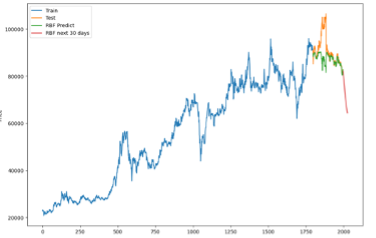
\includegraphics[width=\linewidth]{bibliography/SVR_VCB91.png}
%     \caption{SVR model's result with 9:1 splitting proportion}
%     \label{fig9}
%   \end{minipage}
% \end{figure}
% \begin{figure}[H]
%   \centering
%   \begin{minipage}{0.8\linewidth}
%     \centering
%     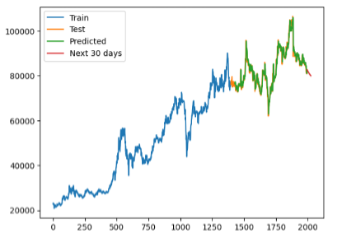
\includegraphics[width=\linewidth]{bibliography/GRU_VCB73.png}
%     \caption{GRU model's result with 7:3 splitting proportion}
%     \label{fig10}
%   \end{minipage}
% \end{figure}
% \begin{figure}[H]
%   \centering
%   \begin{minipage}{0.8\linewidth}
%     \centering
%     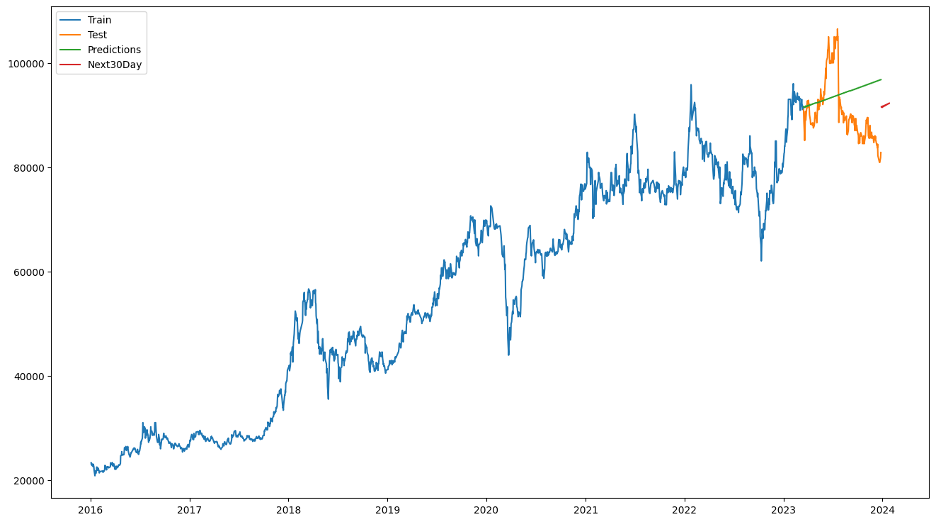
\includegraphics[width=\linewidth]{bibliography/ARIMA_VCB91.png}
%     \caption{ARIMA model's result with 9:1 splitting proportion}
%     \label{fig11}
%   \end{minipage}
% \end{figure}
% \begin{figure}[H]
%   \centering
%   \begin{minipage}{0.8\linewidth}
%     \centering
%     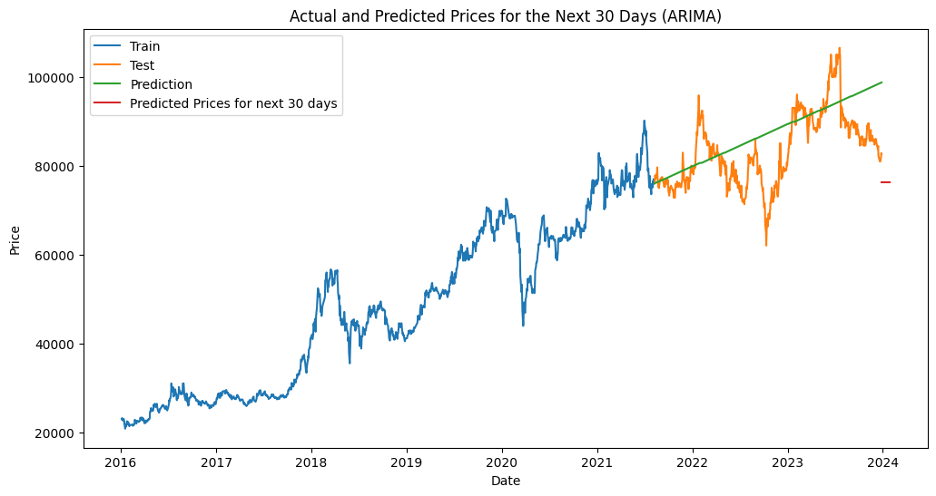
\includegraphics[width=\linewidth]{bibliography/SARIMA_VCB73.png}
%     \caption{SARIMA model's result with 7:3 splitting proportion}
%     \label{fig12}
%   \end{minipage}
% \end{figure}
% \begin{figure}[H]
%   \centering
%   \begin{minipage}{0.8\linewidth}
%     \centering
%     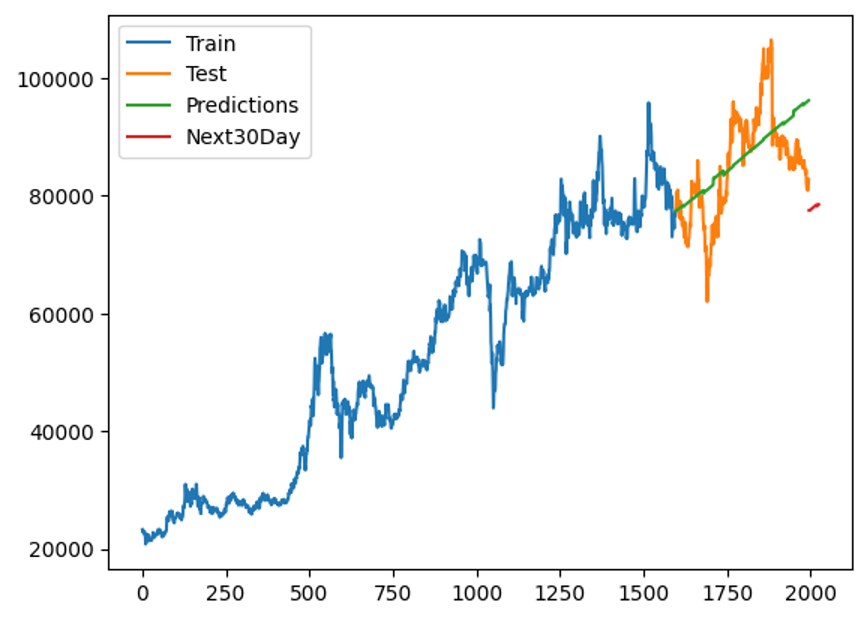
\includegraphics[width=\linewidth]{bibliography/DLM_VCB82.png}
%     \caption{DLM model's result with 8:2 splitting proportion}
%     \label{fig13}
%   \end{minipage}
% \end{figure}
% \begin{figure}[H]
%   \centering
%   \begin{minipage}{0.8\linewidth}
%     \centering
%     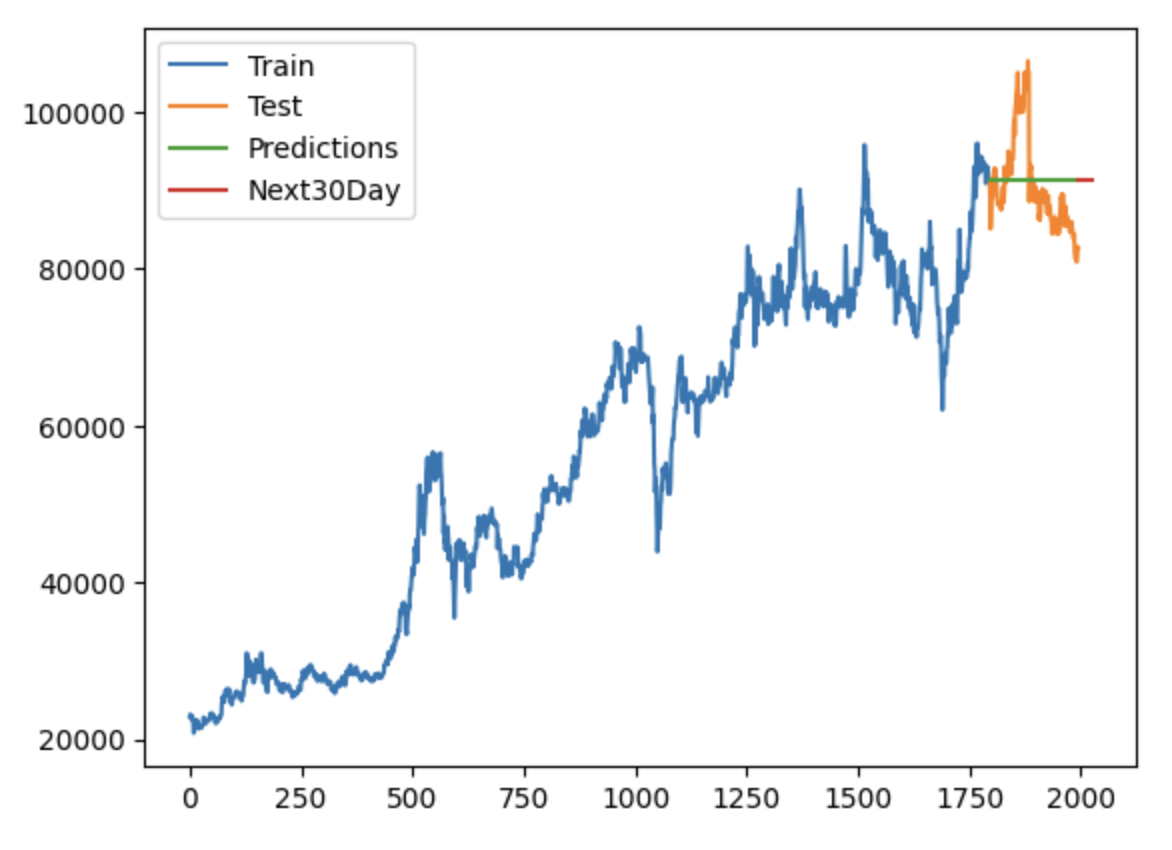
\includegraphics[width=\linewidth]{bibliography/ETS_VCB91.png}
%     \caption{SES model's result with 9:1 splitting proportion}
%     \label{fig14}
%   \end{minipage}
% \end{figure}
% \begin{figure}[H]
%   \centering
%   \begin{minipage}{0.8\linewidth}
%     \centering
%     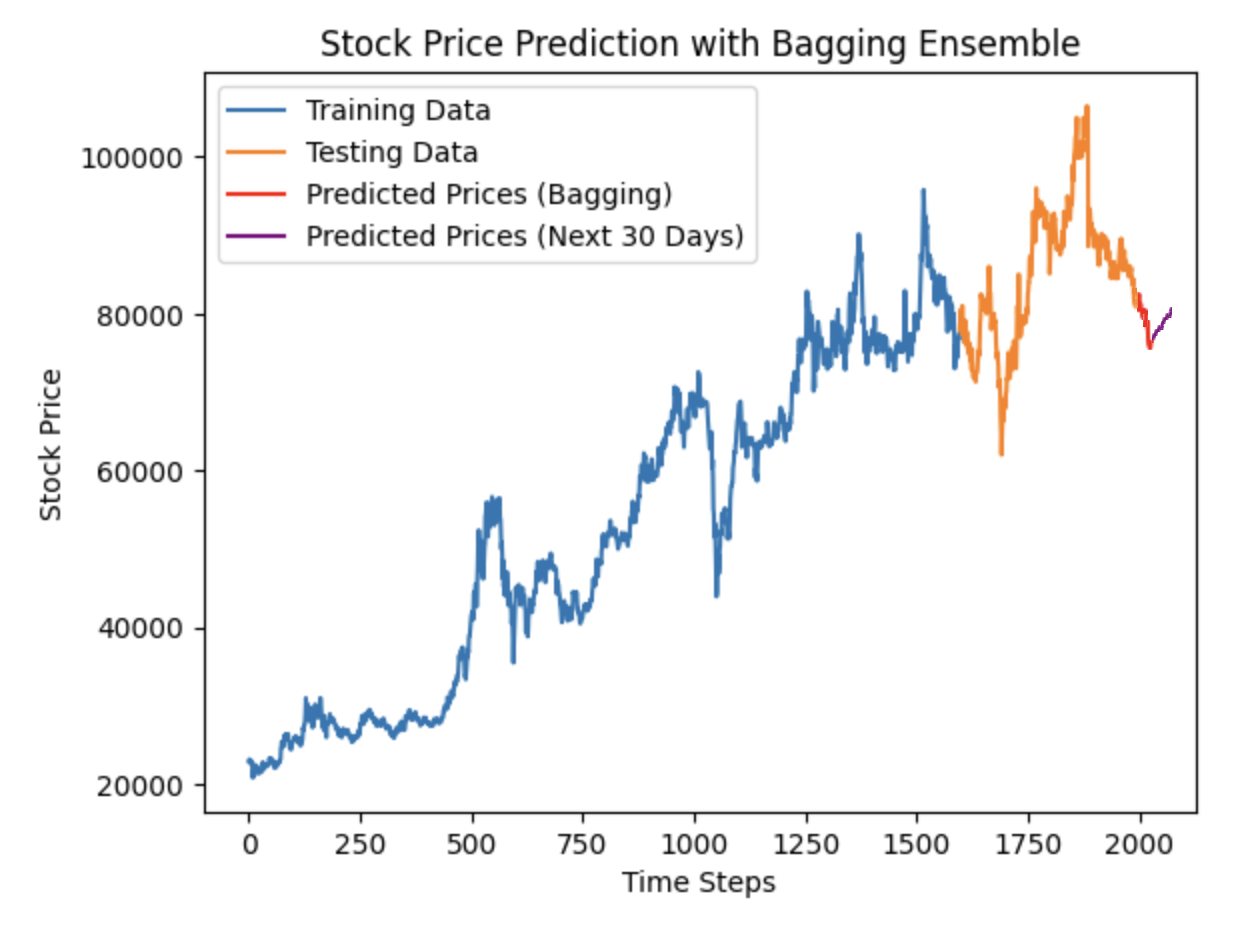
\includegraphics[width=\linewidth]{bibliography/baggingGRU_vcb.png}
%     \caption{Bagging-GRU model's result with 8:2 splitting proportion}
%     \label{bagginggru}
%   \end{minipage}
% \end{figure}
\subsection{DIG dataset} 
% \begin{table}[H]
%     \centering
%     \begin{tabular}{|c|c|c|c|c|}
%          \hline
%          \multicolumn{5}{|c|}{\textbf{MBB Dataset's Evaluation}}\\
%          \hline
%          \centering Model & Training:Testing & RMSE & MAPE (\%) & MSLE\\
%          \hline
%          \multirow{2}{*}{LN} & \textbf{7:3}&\textbf{4983.47}&\textbf{17.44}&\textbf{0.058} \\ & 8:2 &  5293.6 & 26.28 & 0.063 \\ & 9:1&4894.46&25.85&0.055\\
%          \hline
%          \multirow{2}{*}{SVR} & 7:3&977.55&1.76&0.002 \\ & 8:2&242.75&0.89&0.0002 \\ & \textbf{9:1} & \textbf{162.85} & \textbf{0.75} & \textbf{0.00008}\\
%          \hline
%          \multirow{2}{*}{GRU} & 7:3&454.9923&1.54&0.0005 \\ &  8:2&388.5658&1.406&	0.0005 \\ & \textbf{9:1} & \textbf{373.744} & \textbf{1.36} & \textbf{0.00038}\\
%          \hline
%          \multirow{2}{*}{ARIMA} & 7:3 & 9682.514 & 43.586 & 0.161 \\ & 8:2 & 7136.268 & 36.166 & 0.106 \\ & \textbf{9:1} & \textbf{1139.476} & \textbf{4.57} & \textbf{0.004}\\
%          \hline
%          \multirow{2}{*}{SARIMA} & 7:3 & 9693.439 & 43.648&0.162 \\ &8:2 & 4564.211 & 23.154 & 0.05 \\ &  \textbf{9:1} &  \textbf{1137.416} &  \textbf{4.564} &  \textbf{0.004}\\
%          \hline
%          \multirow{2}{*}{DLM} & 7:3 & 9428.531 & 41.483 & 0.154 \\ & 8:2 & 7054.485 & 34.819 & 0.102\\ & \textbf{9:1} & \textbf{1297.301} & \textbf{5.744} & \textbf{0.005}\\
%          \hline
%          \multirow{2}{*}{SES} & 7:3 &  4988.1456 & 22.7511 & 0.0546 \\ & 8:2 & 4659.5801 & 23.6876 & 0.0516 \\ & \textbf{9:1} &  \textbf{1137.4155} &	\textbf{4.5635} & 	\textbf{0.0036} \\
%          \hline
%          \multirow{2}{*}{BaggingGRU} & 7:3 & 941.7588 &  1.7384 &  0.0005 \\ & 8:2 & 939.7588 &  1.6546 &  0.0005 \\ & \textbf{9:1} & \textbf{936.8374} & \textbf{1.6273} & \textbf{0.0005}\\
%          \hline
%     \end{tabular}
%     \caption{MBB Dataset's Evaluation}
%     \label{mbbresult}
% \end{table}

% \begin{figure}[H]
%   \centering
%   \begin{minipage}{0.8\linewidth}
%     \centering
%     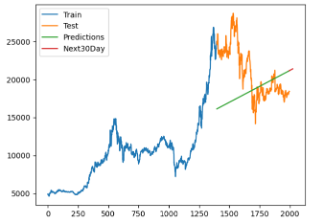
\includegraphics[width=\linewidth]{bibliography/LN_MBB73.png}
%     \caption{Linear model's result with 7:3 splitting proportion}
%     \label{fig15}
%   \end{minipage}
% \end{figure}
% \begin{figure}[H]
%   \centering
%   \begin{minipage}{0.8\linewidth}
%     \centering
%     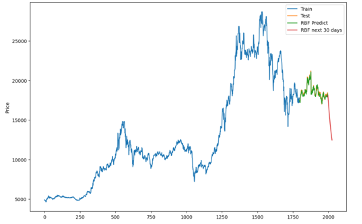
\includegraphics[width=\linewidth]{bibliography/SVR_MBB91.png}
%     \caption{SVR model's result with 9:1 splitting proportion}
%     \label{fig16}
%   \end{minipage}
% \end{figure}
% \begin{figure}[H]
%   \centering
%   \begin{minipage}{0.8\linewidth}
%     \centering
%     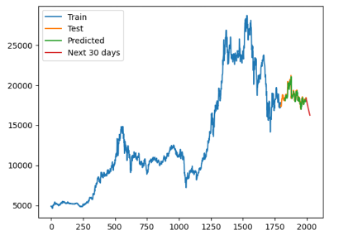
\includegraphics[width=\linewidth]{bibliography/GRU_MBB91.png}
%     \caption{GRU model's result with 9:1 splitting proportion}
%     \label{fig17}
%   \end{minipage}
% \end{figure}
% \begin{figure}[H]
%   \centering
%   \begin{minipage}{0.8\linewidth}
%     \centering
%     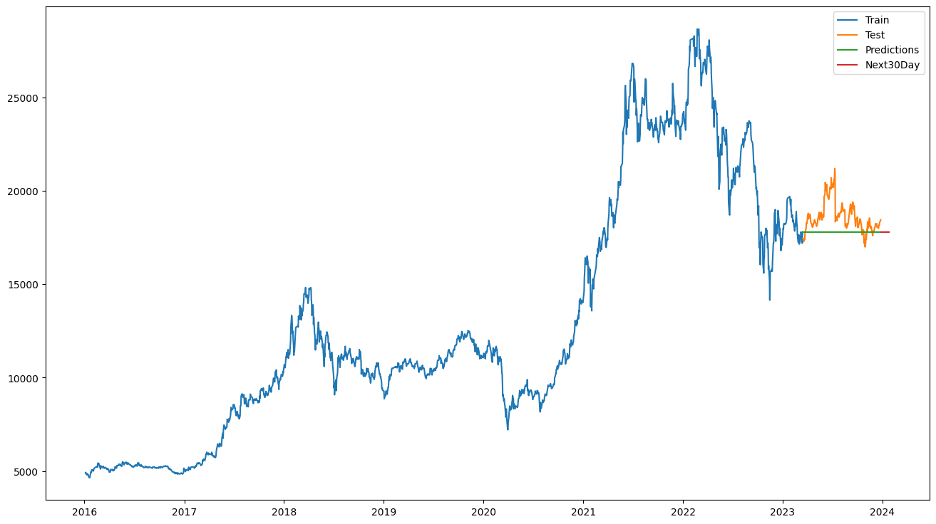
\includegraphics[width=\linewidth]{bibliography/ARIMA_MBB91.png}
%     \caption{ARIMA model's result with 9:1 splitting proportion}
%     \label{fig18}
%   \end{minipage}
% \end{figure}
% \begin{figure}[H]
%   \centering
%   \begin{minipage}{0.8\linewidth}
%     \centering
%     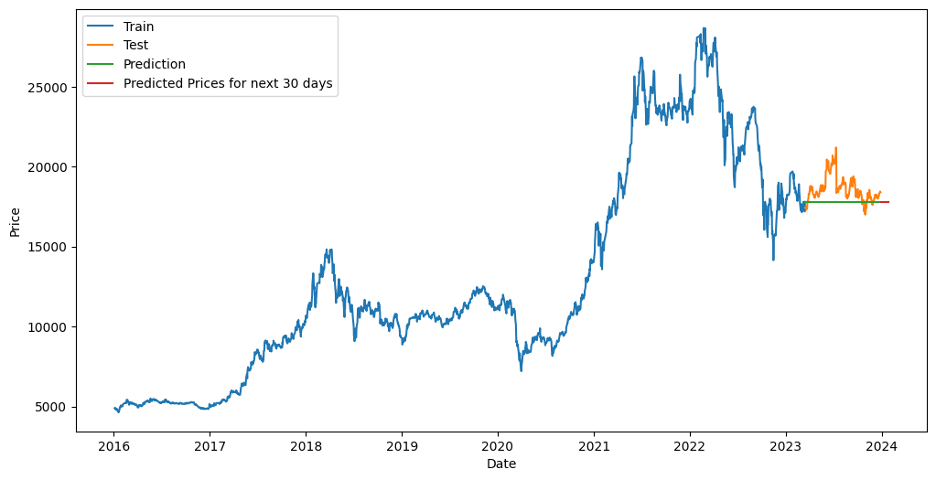
\includegraphics[width=\linewidth]{bibliography/SARIMA_MBB91.png}
%     \caption{SARIMA model's result with 9:1 splitting proportion}
%     \label{fig19}
%   \end{minipage}
% \end{figure}
% \begin{figure}[H]
%   \centering
%   \begin{minipage}{0.8\linewidth}
%     \centering
%     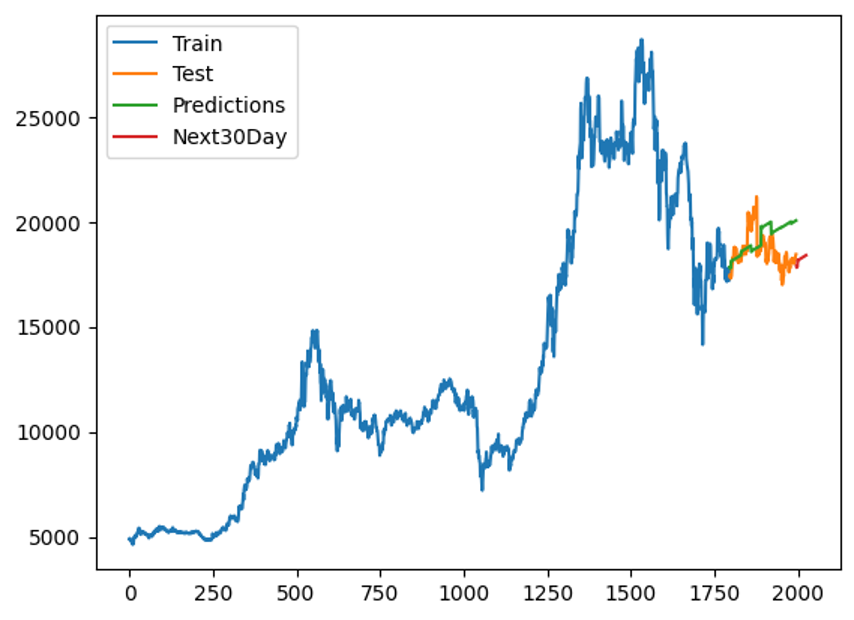
\includegraphics[width=\linewidth]{bibliography/DLM_MBB91.png}
%     \caption{DLM model's result with 9:1 splitting proportion}
%     \label{fig20}
%   \end{minipage}
% \end{figure}
% \begin{figure}[H]
%   \centering
%   \begin{minipage}{0.8\linewidth}
%     \centering
%     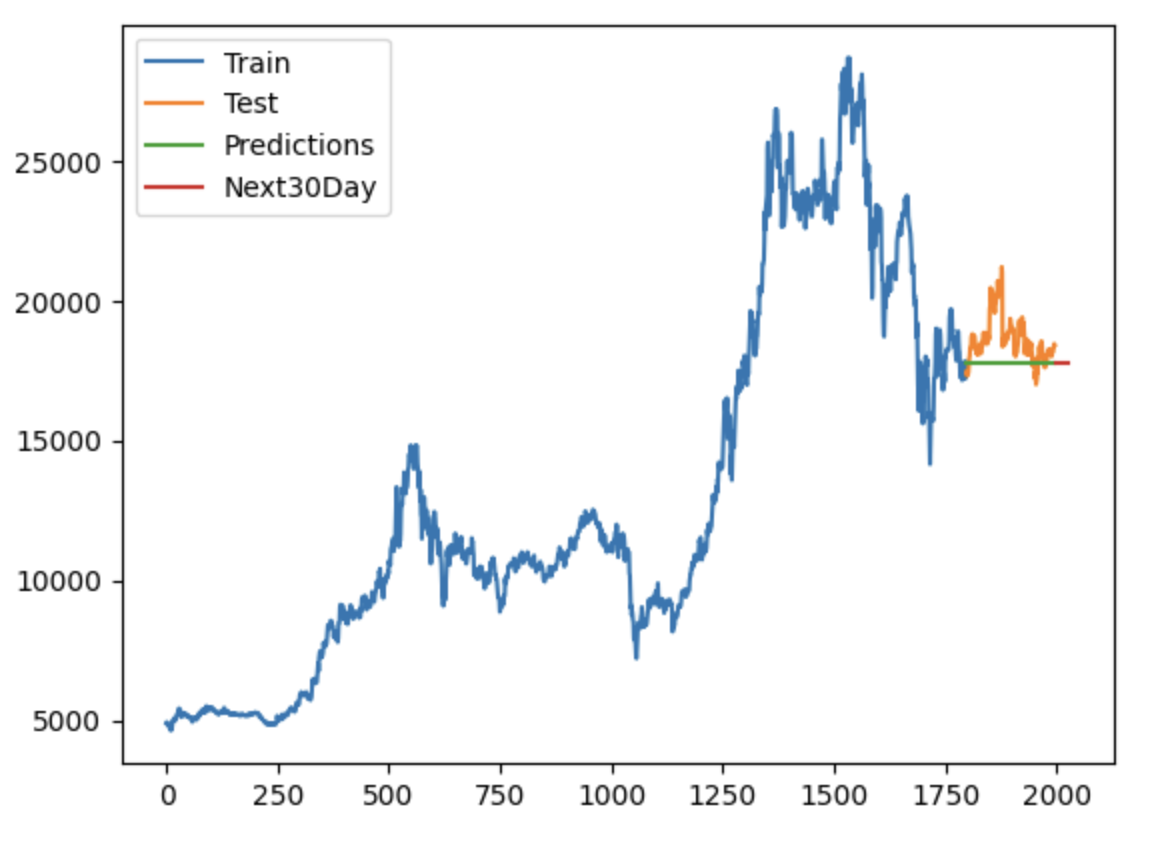
\includegraphics[width=\linewidth]{bibliography/ETS_MBB91.png}
%     \caption{SES model's result with 9:1 splitting proportion}
%     \label{fig21}
%   \end{minipage}
% \end{figure}
% \begin{figure}[H]
%   \centering
%   \begin{minipage}{0.8\linewidth}
%     \centering
%     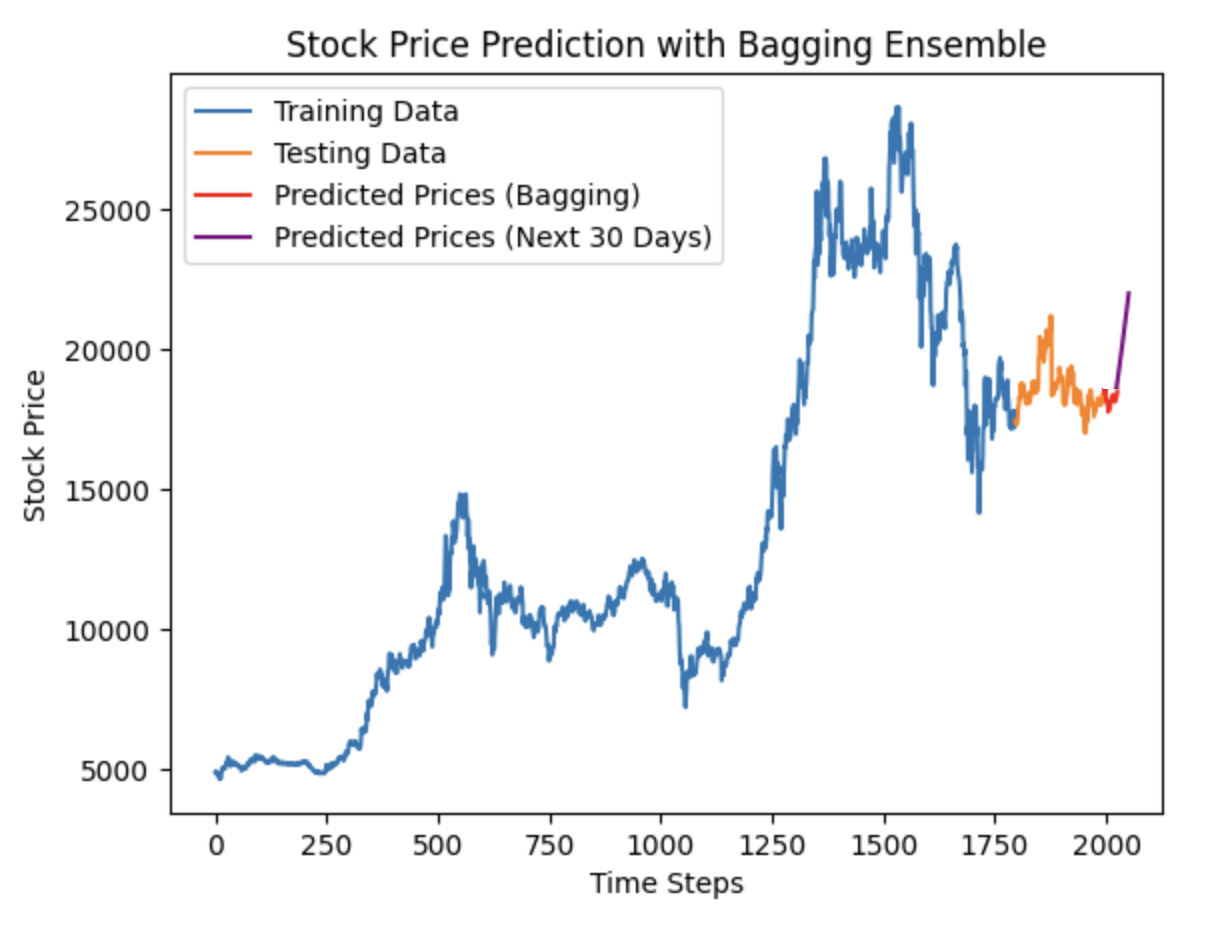
\includegraphics[width=\linewidth]{bibliography/baggingGRU_MBB.png}
%     \caption{Bagging-GRU model's result with 9:1 splitting proportion}
%     \label{mbbbggg}
%   \end{minipage}
% \end{figure}
\subsection{NVL dataset} 
% \begin{table}[H]
%     \centering
%     \begin{tabular}{|c|c|c|c|c|}
%          \hline
%          \multicolumn{5}{|c|}{\textbf{Dataset's Evaluation}}\\
%          \hline
%          \centering Model & Training:Testing & RMSE & MAPE (\%) & MSLE\\
%          \hline
%          \multirow{2}{*}{LN} & 7:3 & 5690.9 & 13.03 & 0.021 \\ & 8:2 & 4904.44 & 10.28 & 0.016 \\ & \textbf{9:1} & \textbf{2859.97} & \textbf{5.49} & \textbf{0.004} \\
%          \hline
%          \multirow{2}{*}{SVR} & 7:3 & 5212.21 & 7.55 & 0.016 \\ & 8:2 & 1014.97 & 1.62 & 0.0005 \\ & \textbf{9:1} & \textbf{822.63} & \textbf{1.26} & \textbf{0.0003}\\
%          \hline
%          \multirow{2}{*}{GRU} & 7:3 & 916.692 & 1.67 & 0.00055 \\ &  8:2 & 948.341 & 1.74 & 0.00057 \\ & \textbf{9:1} &. \textbf{761.754} & \textbf{1.21} & \textbf{0.0003}\\
%          \hline
%          \multirow{2}{*}{ARIMA} & 7:3 & 7847.594 & 15.278 & 0.041 \\ & 8:2 & 7501.223 & 15.14 & 0.036 \\ & \textbf{9:1} & \textbf{3371.058} & \textbf{6.414} & \textbf{0.006}\\
%          \hline
%          \multirow{2}{*}{SARIMA} & 7:3 & 7849.75 & 15.29 & 0.04 \\ &8:2 &7501.73 & 15.15 & 0.04 \\ &  \textbf{9:1} & \textbf{3373.34} & \textbf{6.43} & \textbf{0.006}\\
%          \hline
%          \multirow{2}{*}{DLM} & 7:3 & 4288.68 & 8.641 & 0.012\\ & 8:2 & 3771.703	& 7.756 & 0.009\\ & \textbf{9:1} & \textbf{3617.388} & \textbf{6.446} & \textbf{0.007}\\
%          \hline
%          \multirow{2}{*}{SES} & 7:3 &  7849.6833 & 15.2872 & 0.0407 \\ & 8:2 & 7502.4992 & 15.1483 & 0.0357 \\ & \textbf{9:1} &  \textbf{3342.8102} &	\textbf{6.3561} & 	\textbf{0.0057} \\
%          \hline
%          \multirow{2}{*}{BaggingGRU} & 7:3 & 941.7588 &  1.7384 &  0.0005 \\ & 8:2 & 939.7588 &  1.6546 &  0.0005 \\ & \textbf{9:1} & \textbf{936.8374} & \textbf{1.6273} & \textbf{0.0005}\\
%          \hline
%     \end{tabular}
%     \caption{BIDV Dataset's Evaluation}
%     \label{mbbresult}
% \end{table}

% \begin{figure}[H]
%   \centering
%   \begin{minipage}{0.8\linewidth}
%     \centering
%     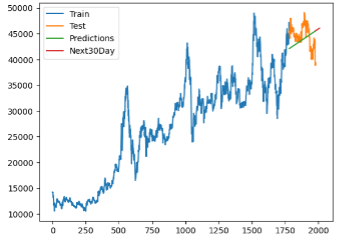
\includegraphics[width=\linewidth]{bibliography/LN_BIDV91.png}
%     \caption{Linear model's result with 9:1 splitting proportion}
%     \label{fig22}
%   \end{minipage}
% \end{figure}
% \begin{figure}[H]
%   \centering
%   \begin{minipage}{0.8\linewidth}
%     \centering
%     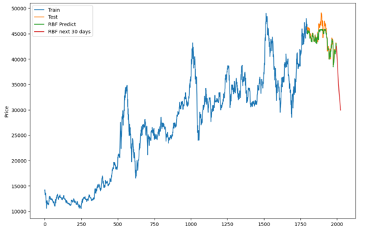
\includegraphics[width=\linewidth]{bibliography/SVR_BIDV91.png}
%     \caption{SVR model's result with 9:1 splitting proportion}
%     \label{fig23}
%   \end{minipage}
% \end{figure}
% \begin{figure}[H]
%   \centering
%   \begin{minipage}{0.8\linewidth}
%     \centering
%     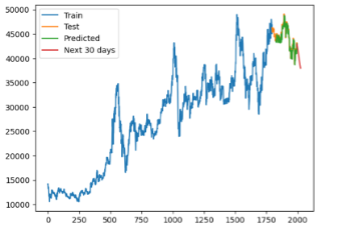
\includegraphics[width=\linewidth]{bibliography/GRU_BIDV91.png}
%     \caption{GRU model's result with 9:1 splitting proportion}
%     \label{fig24}
%   \end{minipage}
% \end{figure}
% \begin{figure}[H]
%   \centering
%   \begin{minipage}{0.8\linewidth}
%     \centering
%     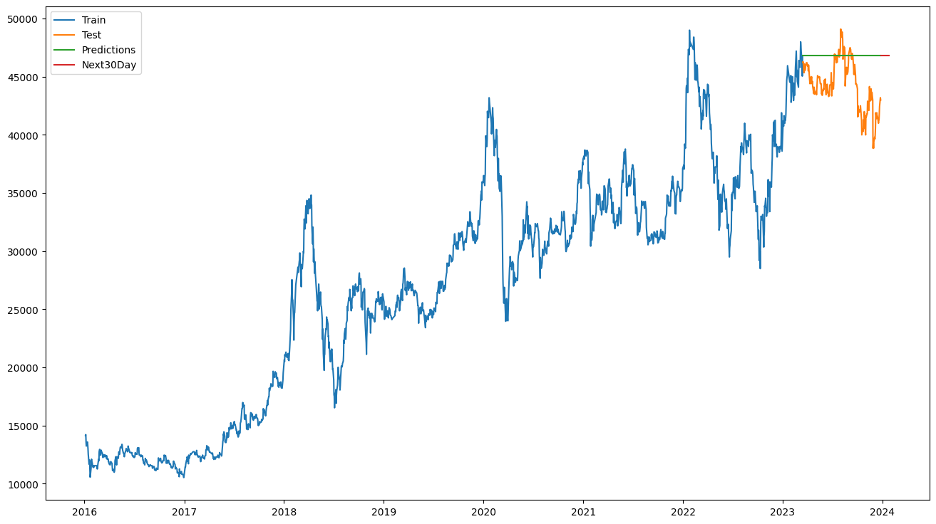
\includegraphics[width=\linewidth]{bibliography/ARIMA_BIDV91.png}
%     \caption{ARIMA model's result with 9:1 splitting proportion}
%     \label{fig25}
%   \end{minipage}
% \end{figure}
% \begin{figure}[H]
%   \centering
%   \begin{minipage}{0.8\linewidth}
%     \centering
%     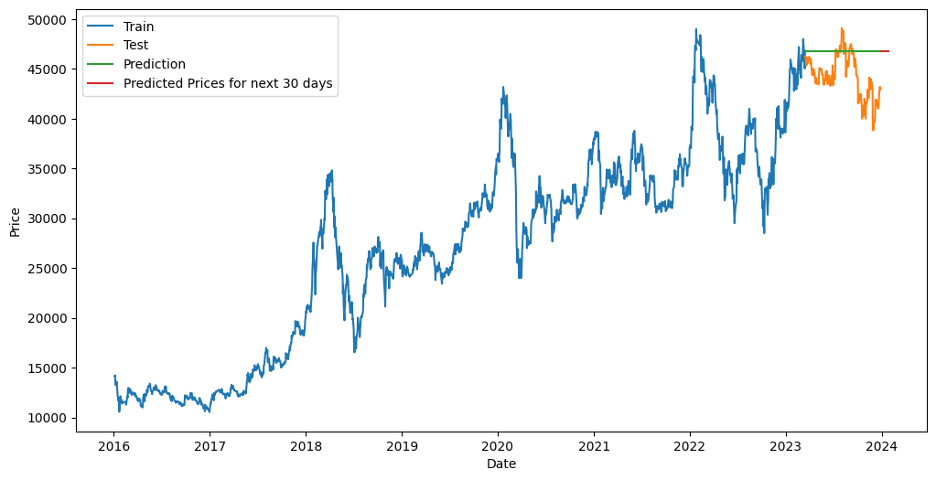
\includegraphics[width=\linewidth]{bibliography/SARIMA_BIDV91.png}
%     \caption{SARIMA model's result with 9:1 splitting proportion}
%     \label{fig26}
%   \end{minipage}
% \end{figure}
% \begin{figure}[H]
%   \centering
%   \begin{minipage}{0.8\linewidth}
%     \centering
%         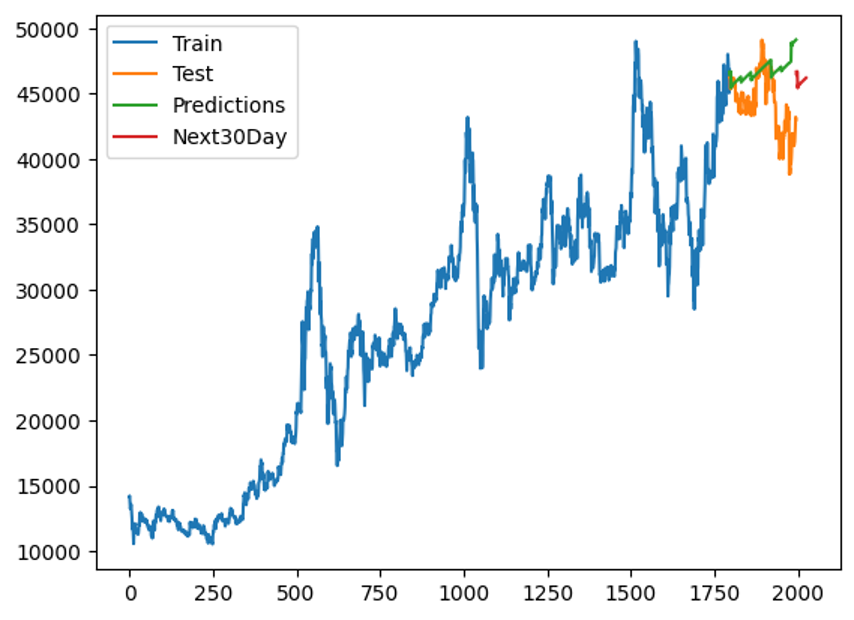
\includegraphics[width=\linewidth]{bibliography/BIDV_DLM91.png}
%     \caption{DLM model's result with 9:1 splitting proportion}
%     \label{fig27}
%   \end{minipage}
% \end{figure}
% \begin{figure}[H]
%   \centering
%   \begin{minipage}{0.8\linewidth}
%     \centering
%         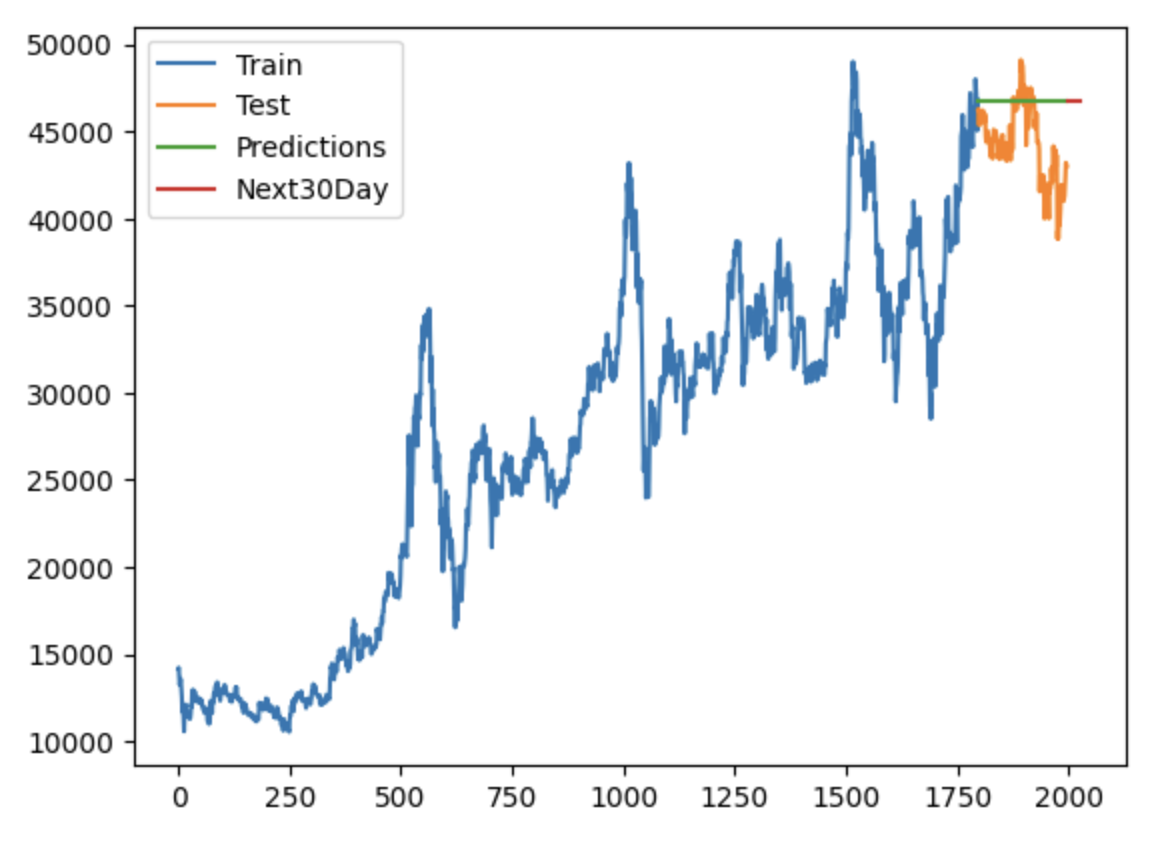
\includegraphics[width=\linewidth]{bibliography/ETS_BIDV91.png}
%     \caption{SES model's result with 9:1 splitting proportion}
%     \label{fig28}
%   \end{minipage}
% \end{figure}
% \begin{figure}[H]
%   \centering
%   \begin{minipage}{0.8\linewidth}
%     \centering
%         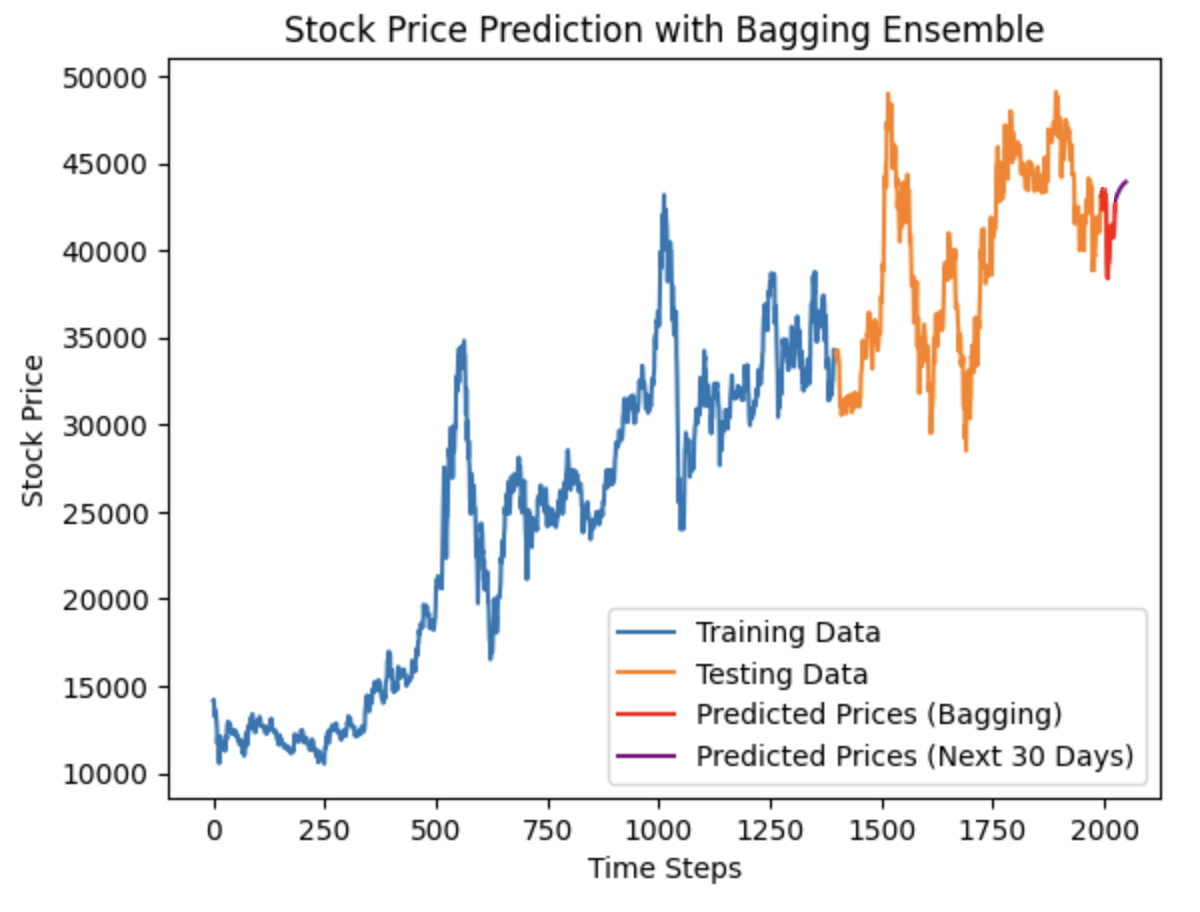
\includegraphics[width=\linewidth]{bibliography/baggingGRU_BIDV.png}
%     \caption{Bagging-GRU model's result with 7:3 splitting proportion}
%     \label{fig28}
%   \end{minipage}
% \end{figure}
\section{Conclusion}
\subsection{Summary}
% In the achievement of forecasting stock prices, the exploration of diverse methodologies, ranging from traditional statistical models to advanced machine learning algorithms, has been aimed. Among the performed models, Linear Regression (LR), Auto Regressive Integrated Moving Average (ARIMA), Support Vector Regression (SVR), Seasonal Auto Regression Integrated Moving Average (SARIMA), Dynamic Linear Model (DLM), Bagging – GRU, and Simple Exponential Smoothing (SES), it becomes evident that Support Vector Regression (SVR), Gated Recurrent Unit (GRU), and Bagging GRU emerge as the most promising and effective models for predicting stock prices.\\
% The intricacies of stock price forecasting, rooted in the complexity and unpredictability of financial markets, demand models that can capture nuanced patterns and relationships within the data. Support Vector Regression (SVR) showcases its efficacy in handling intricate relationships, providing robust predictions. Gated Recurrent Unit (GRU) models, with their ability to capture sequential dependencies, exhibit notable performance in forecasting stock prices. The introduction of ensemble learning through Bagging GRU further refines the predictive capabilities, offering a collective insight that surpasses individual models.\\
% As evidenced by the evaluation metrics, including RMSE, MAPE, and MSLE, the SVR, GRU, and Bagging GRU models consistently demonstrate superior performance across various aspects of forecasting accuracy. Their adaptability to handle the inherent uncertainties of stock markets positions them as formidable tools for investors and analysts seeking reliable predictions.
\subsection{Future Considerations}
% In our future research, it is crucial to prioritize further optimization of the previously mentioned models. This optimization effort should specifically focus on:\\
% \indent\textbullet\ Enhancing the accuracy of the model. While the above algorithms have demonstrated promising results in predicting stock prices, there is a need to further improve the model's accuracy to ensure more precise forecasting outcomes.\\
% \indent\textbullet\ Exploring alternative machine learning algorithms or ensemble techniques. Ensemble techniques, such as combining multiple models or using various ensemble learning methods, can also improve the robustness and accuracy of the forecasts.\\
% \indent\textbullet\ Researching new forecasting models. The field of forecasting continuously evolves, with new algorithms and models being researched and developed. It is crucial to stay updated with these approaches and explore new forecasting models that offer improved accuracy and performance. \\
% By continuously exploring and incorporating new features, data sources, and modeling techniques, we can strive for ongoing optimization of the forecasting models and enhance their ability to predict stock prices with greater precision and reliability.

\section*{Acknowledgment}
\addcontentsline{toc}{section}{Acknowledgment}
First and foremost, we would like to express our sincere gratitude to \textbf{Assoc. Prof. Dr. Nguyen Dinh Thuan} and \textbf{Mr. Nguyen Minh Nhut} for their exceptional guidance, expertise, and invaluable feedback throughout the research process. Their mentorship and unwavering support have been instrumental in shaping the direction and quality of this study. Their profound knowledge, critical insights, and attention to detail have significantly contributed to the success of this research.
\\This research would not have been possible without the support and contributions of our mentors. We would like to extend our heartfelt thanks to everyone involved for their invaluable assistance, encouragement, and belief in our research. Thank you all for your invaluable assistance and encouragement.

%% UNCOMMENT these lines below (and remove the 2 commands above) if you want to embed the bibliografy.
\begin{thebibliography}{00}

% \bibitem{b1} V. Gururaj,  ''Stock Market Prediction using Linear Regression and Support Vector Machines'' vol. 14, no. 8, 2019.
% \bibitem{b2} YURTSEVER, M., 2021. Gold price forecasting using LSTM, Bi-LSTM and GRU. Avrupa Bilim ve Teknoloji Dergisi, (31), pp.341-347.
% \bibitem{b3} Kishanna, H., RamaParvathyb, L. and SIMATS, C., 2022. A Novel Approach for Correlation Analysis on FBProphet to Forecast Market Gold Rates with Linear Regression.
% \bibitem{b4} A. O. A. A. A. Ariyo, ``Stock Price Prediction Using the ARIMA Model'' ,2014. [Online]. Available:https://ieeexplore.ieee.org/document/7046047..
% \bibitem{b5} M. S. S. S. A. F. K. Senthamarai Kannan, ``Comparison Of Fuzzy Time Series And ARIMA''August 2019. [Online]. Available:https://www.ijstr.org/final-print/aug2019/Comparison-Of-Fuzzy-Time-Series-And-Arima-Model.pdf. [Accessed 19 June 2023].
% \bibitem{b6} B. M. Henrique, V. A. Sobrero, and H. Kimura, ''Stock price prediction using support vector regression on daily and up to the minute prices'' J. Finance Data Sci., vol. 4,no. 3, pp. 183–201, Sep. 2018, doi: 10.1016/j.jfds.2018.04.003. 5
% \bibitem{b7}Avner Abrami, Aleksandr Y. Aravkin, Younghun Kim, ''Time Series Using Exponential Smoothing Cells'', 9 June 2017.
% \bibitem{b8}  Professor Thomas B. Fomby, ''Exponential Smoothing Models'', June 2008.
% \bibitem{b9} Bauer, E., Kohavi, R. ''An Empirical Comparison of Voting Classification Algorithms: Bagging, Boosting, and Variants''. Machine Learning 36, 105–139 (1999). https://doi.org/10.1023/A:1007515423169.
% \bibitem{b10} Buja, A., and Stuetzle, W. ''Observations on bagging''. University of Pennsylvania and University of Washington, Seattle. 2002.
% \bibitem{b11} B. M. Henrique, V. A. Sobrero, and H. Kimura, ``Comparison Of Fuzzy Time Series And ARIMA'', August 2019. Available:https://www.ijstr.org/final-print/aug2019/Comparison-Of-Fuzzy-Time-Series-And-Arima-Model.pdf. [Accessed 19 June 2023]. 4
% \bibitem{b12} Jason Brownlee, ``How to Create an ARIMA Model for Time Series Forecasting in Python'', November 18, 2023. Available:https://www.ijstr.org/final-print/aug2019/Comparison-Of-Fuzzy-Time-Series-And-Arima-Model.pdf. 
% \bibitem{b13} Jason Brownlee, ``A Gentle Introduction to SARIMA for Time Series Forecasting in Python'', August 21, 2019. 
%\bibitem{b14} Alexandra M. Schmidt and Hedibert F. Lopes, ''Dynamic models'', 2019. 
%\bibitem{b15} Timothy O. Hodson, ''Root-mean-square error (RMSE) or mean absolute error (MAE): when to use them or not'', 2022, https://doi.org/10.5194/gmd-15-5481-2022.
%\bibitem{b16} Priya Pedamkar,''Support Vector Regression'', March 24, 2023. Retrieved from \(https://www.educba.com/support-vector-regression/?fbclid=IwAR0ibzdmqpaaDKq2-Q4JRcjxQcVt-C7TrHNEc90q_tCSrn8rds9x2AG8Y78\)
%\bibitem{b17} Seok-Ho Han, Husna Mutahira, Hoon-Seok Jang, "Prediction of Sensor Data in a Greenhouse for Cultivation of Paprika Plants Using a Stacking Ensemble for Smart Farms", Applied Sciences, vol.13, no.18, pp.10464, 2023.
\end{thebibliography}
%%%%%%%%%%%%%%%


\EOD

\end{document}
